\section{Computer Arithmetic}

We often want to work with the real number system, which consists of all 
integers, rational and irrational numbers
\begin{equation*}
  2, \sqrt{2}, e, \pi, 10^6, \text{ etc.} 
\end{equation*}
Because we have a finite space limitation for numbers, 
\textbf{not all numbers can be represented exactly.} This can cause problems
with arithmetic.

\subsection{Bases - Binary and Decimal}

We typically use the decimal (base 10) system, e.g.
\begin{equation*}
  427.325 = 4 \times 10^2 + 2 \times 10^1 + 7 \times 10^{0} + 3 \times 10^{-1}+\dots
\end{equation*}
However, when we work with a computer, we use the binary (base 2) system:
\begin{equation*}
  (1001.11101)_2 = 1\times 2^3 + 0\times 2^2 + 0\times 2 + 1\times 2^0 + 1\times 2^{-1} + 1\times 2^{-2} + 1\times 2^{-3} +\dots
\end{equation*}
In this class, we will only be working in the decimal system in order to make
computations simpler, since the application of concepts is identical.

\subsection{Base Conversion and Error}

Because it is impossible to represent some finite decimal fractions in binary,
we will (definitely) encounter \textbf{error} when converting from base-10 to
base-2. In the following example, we will convert $\frac{1}{10}$ to binary, and
show how there exists some numbers which cannot be represented exactly within 
the binary floating-point system.

% Notice that conversion from base-10 to base-2 can lead to errors. It is 
% impossible to represent some finite decimal fractions in binary.

\subsubsection{Example}

To convert a decimal fraction like $\frac{1}{10}$ into its binary 
representation, we repeatedly multiply the fractional part by $2$ and extract
the integer part at each step.

We begin with $1/10 = 0.1_{10}$, and assume $0.1_{10} = (a_1.a_2a_3\dots
a_n)_2$.
\[
\frac{1}{10} = 0.1_{10} = (0.a_1a_2a_3\dots a_n)_{2}
\]

Multiply by $2$:
\[
2 \times 0.1 = 0.2 = (a_1.a_2a_3\dots)_2
\]

Keep the fractional part and repeat:
\begin{align*}
  &a_1 = \lfloor 0.2 \rfloor = 0 \\
  2 \times 0.2 = 0.4 \implies &a_2 = \lfloor 0.4 \rfloor = 0 \\
  2 \times 0.4 = 0.8 \implies &a_3 = \lfloor 0.8 \rfloor = 0 \\
  2 \times 0.8 = 1.6 \implies &a_4 = \lfloor 1.6 \rfloor = 1 \\
  1.6 - 1 &= 0.6 \\
  2 \times 0.6 = 1.2 \implies &a_5 = \lfloor 1.2 \rfloor = 1 \\
  1.2 - 1 &= 0.2
\end{align*}

We have now returned to $0.2$, which was the value after the very first 
multiplication. This means the process will repeat indefinitely. Thus, the 
binary representation of $\frac{1}{10}$ is:
\[
  \frac{1}{10} = (0.0\mathbf{0011}00110011\dots)_2
\]
The repeating part is \textbf{0011}\dots, and this pattern continues forever. 
Using a finite number of digits, $\frac{1}{10}$ \textbf{cannot} be represented
exactly in binary. Just as $\frac{1}{3} = 0.\overline{3}$ cannot
be perfectly represented in decimal, the same is true for $\frac{1}{10}$ in
binary. This is why certain decimal fractions lead to rounding errors in binary-
based floating-point arithmetic.

\section{Hypothetical Storage Scheme (32-bit)}

We will use a hypothetical decimal computer since the concept is identical.
(By the way, this is very close to 
\ulhref{https://en.wikipedia.org/wiki/IEEE_754}{IEEE-754} floating point
representation, except that we are using a decimal representation instead of
binary.)

Suppose we have the decimal number $423.7$. Since we always want to represent
numbers in proper scientific notation, we normalize the
\textbf{mantissa}.
We write our number as follows:

\begin{equation*}
  423.7 = +\underbrace{0.4237}_{\text{mantissa}} \times 10^{+3}
\end{equation*}
Notice the $+$ is relevant because we require an explicit representation of the
sign of the number. We call the bits following from the decimal point ($4273$) 
the \textbf{mantissa}.
We include 1 bit for the sign, which is $1$ for positive numbers, 1 bit for the
exponent sign, 7 bits for the exponent, and the remaining 23 bits for the
mantissa.

\begin{figure}[h]
  \centering
  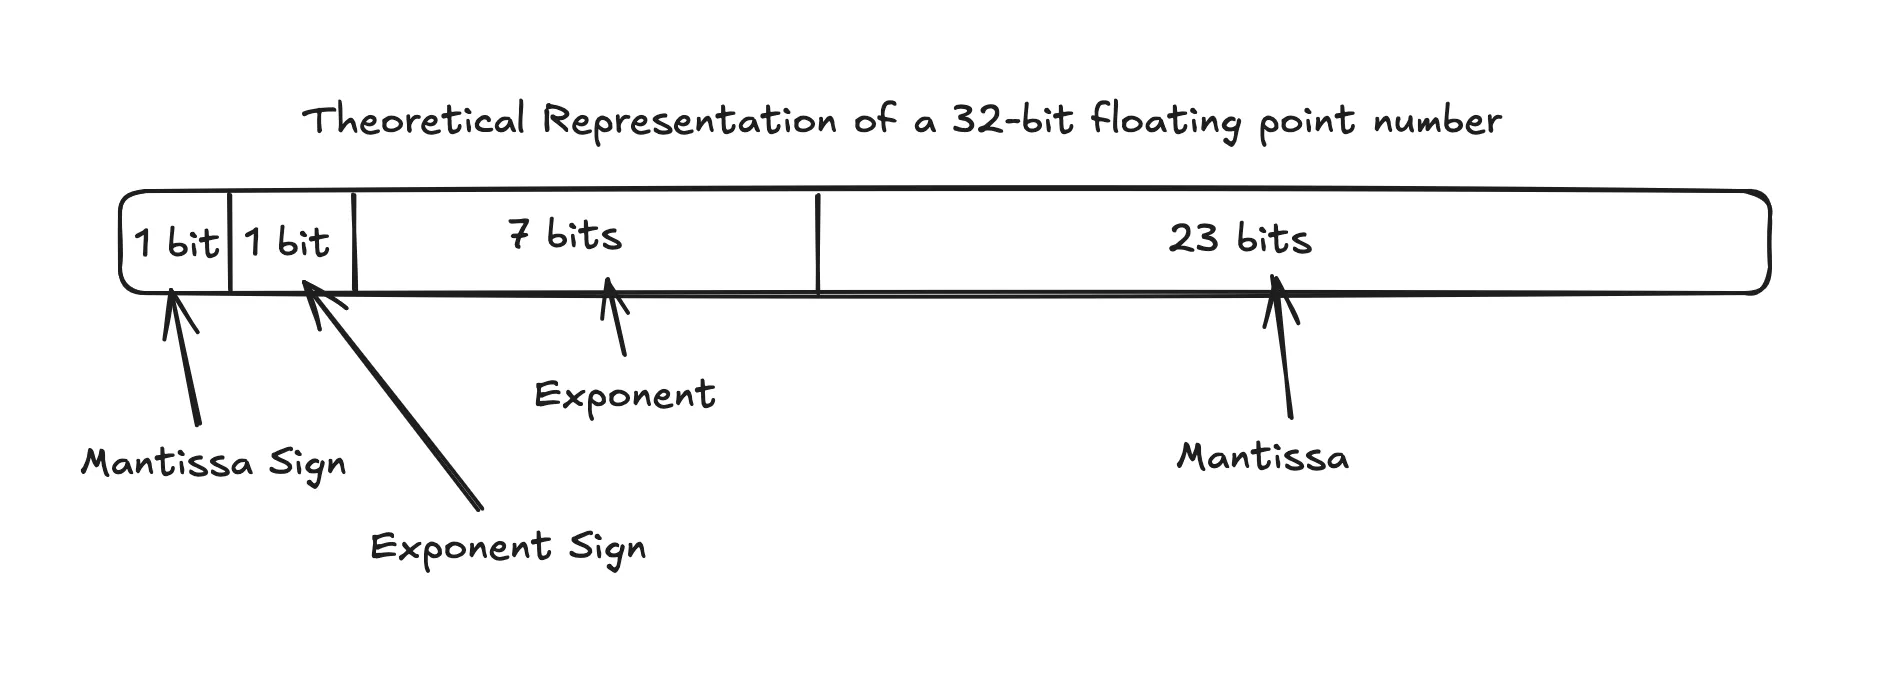
\includegraphics[width=0.8\textwidth]{./assets/fake_ieee754.png}
  \caption{Hypothetical Storage Scheme (32-bit)}
\end{figure}

\subsection{Problems with Floating Point}
\noindent
\begin{minipage}{\textwidth}
Because our storage format is finite, the biggest problems we will encounter
are:
\begin{enumerate}
  \item \textbf{bit overflow}: the maximum magnitude of our exponent (in binary)
    is \textbf{127}, so our number can only range from $2^{-127}$ to $2^{+127}$.
  \item \textbf{rounding error}: because our mantissa only has 23 bits of 
    precision, the precision will decrease as our numbers get larger because we 
    use exponentiation to represent the actual number.
\end{enumerate}
\end{minipage}

% Because our storage format is finite, one of the biggest problems we will 
% encounter is \textbf{bit overflow}. The maximum magnitude of our exponent 
% (in binary) is \textbf{127}, so our number can only range from $2^{-127}$ to
% $2^{+127}$. Because our mantissa only has 23 bits of precision, the precision
% will decrease as our numbers get larger because we use exponentiation to 
% represent the actual number.

\subsubsection{Error Example}

Consider the number $2^{25} = 33,554,432$. This number can be represented 
exactly in binary. However, the number $2^{25}+1 = 33,554,433$ cannot be
represented exactly, since it can't fit within the 23 bits of precision available.

From this, we find that all numbers (including fractions) from $2^{25}-1$ 
through $2^{25}+2$ are represented with the same mantissa in binary. Only when 
you reach $2^{25}+3$ does the mantissa change.

\subsubsection{Remarks}

Within IEEE-754-style floating point representation, the
number of representable values within a given exponent is the same, regardless
of the exponent. This may seem obvious, but it's interesting nonetheless. This
comes from the fact that the number of bits in the mantissa is fixed. The
number of representable values is exactly $2\times 2^{23} = 2^{24}$, since each
positive value has a negative counterpart.

\subsubsection{Actual IEEE-754 Floating Point}
There are a few key differences betewen our hypothetical storage scheme and the
actual IEEE-754 specification.

\begin{enumerate}
  \item Instead of an exponent sign bit, IEEE-754 specifies a \textbf{biased
    exponent} which just stores the exponent as an 8-bit unsigned integer and
    interprets it as $2^{e-127}$. \Ex we want $2^{2}$ to be the exponent part of
    our number, so we set the biased exponent to $e=2+127=129$. When we decode
    the number, we multiply the mantissa by $2^{129-127 = 2}$ to get the actual
    number.
  \item The hidden bit (implicit leading 1) is a feature of IEEE-754 that allows
    us to \enquote{fake} 24 bits of mantissa precision. We save a bit by
    specifying the zeroth bit of the mantissa as always being a 1, and we can
    use this fact to save one bit of space.
\end{enumerate}
In IEEE-754, the number is represented as
\[
  (-1)^{s} \times 1.f \times 2^{e-127}
.\]
where $s$ is the sign bit, $f$ is the mantissa, and $e$ is the biased exponent.
